\documentclass{article}

\usepackage[a4paper]{geometry} 
\usepackage[dutch]{babel}
\usepackage{parskip}
\usepackage{amsmath, amssymb, textcomp}
\usepackage{color}
\usepackage{graphicx}
\usepackage{enumerate} 
\usepackage[official]{eurosym}
\usepackage{url}
\usepackage{float}
\usepackage{listings} 
\usepackage{gensymb}
\usepackage[normalem]{ulem}
\usepackage{array,ragged2e}


\title{Searching with data structures}
\author{
		Gerben Aalvanger\\ 
	        	Student-number: 3987051 \\
	        	Utrecht University
			\and
		Erik Visser\\
	        	Student-number: 3470806 \\
	        	Utrecht University
	        	\and
		William Kos\\
	        	Student-number: 3933083\\
	        	Utrecht University\\
	        	\and
		Sam van der Wal\\
	        	Student-number: 3962652\\
	        	Utrecht University}
\date{\today \\Teacher: Peter de Waal}
\begin{document}
\maketitle
\section{Introduction}
Searching values and storing them in memory is a key concept in computer science. For optimal speed and complexity, data is stored in a lot of different data structures, for example a tree or a skip-list. Every data structure has its own advantages, some perform better on insertion, while other perform better on finding a specific value. In this document we will describe how we will compare data structures and actually compare them. We will start by proposing a research question and some sub-questions. Secondly we specify the problem we want to research and the scope of our project. After that we explain our experiments in terms of criteria, test data and scenarios. And last we will show in different ways our test results and compare them to each other and end with a conclusion. 

\section{Research description}
In this research the question "Which data structure has the shortest duration on given actions" has been put central. We have used 4 data structures to get the answer to this question. To get the best insight in this question with 4 data structures we had chosen to take data structures which differ a lot from each other, namely:
\begin{itemize}
\item Lists
\item Balanced trees
\item Hash tables
\item Min-max heaps
\end{itemize}
The list and hash table are both straight forward data structures, but there are multiple implementations possible for balanced trees and min-max heaps. For the balanced tree we had chosen to use the AVL tree because it is similar to the red-black tree, but known to be faster on lookups. The min-max heap implementation we have used in our experiments is the interval heap. Our initial idea was to use the original min-max heap implementation but after implementing this algorithm it turned out that it did not work according to what was described in the paper we found. Therefore the decision was made to use the interval heap since the complexity for the individual actions are the same as with the min-max heap. All the actions used in our research will be described in the next section.

Part of the research was performing statistics on the results gained from the experiments. The focus laid at the average and the standard deviation of the performed actions on special cases. Because the same tests were performed multiple times we have chosen for both the average and the standard deviation to gain a good insight in the overall results retrieved from the experiments. 

\section{Experiment description}
We will separate the experiment in several section:
\subsection{Build}
\label{Build}
In the build we have ``build'' the different datastructures. 
For the build operation we have build from 15 different unsorted datasets, this is divided in datasets of size $10.000, 100.00$ and $1.000.000$, each size occurring 5 times.  For each of these 15 options we have also tested the sorted and reverse sorted set. Each dataset is tested 30 times. This means that we have conducted all tests with 1350 distinct datasets.
\subsection{Search}
We have searched in the pre-build datastructures of section \ref{Build}. The amount of searches is half the amount of elements in the datastructure. All the values of the searches are determined random and are guaranteed to be in the datastructure. Like in the build section we have performed all search-tests 30 times. 

We wanted to know if finding the minimum or maximum through the getMin (see section \ref{getMin}) and getMax (see section \ref{getMax}) methods of the datastructures are faster then searching for the minimum or maximum value with this search method. This test is conducted 1000 times on the datasets described in section \ref{Build}
\subsection{Insert}
We have constructed new datastructures from scratch by repeatedly inserting new elements. Like in section \ref{Build} we have tested the insert actions for 15 sets of elements (set sizes: $10.000, 100.000, 1.000.000$) and each of these tests have been performed 30 times.
\subsection{Delete}
We have performed delete operations on the pre-build datastructures of section \ref{Build}. The amount of deletes is half the amount of elements in the datastructure. All the values of the deletes are determined random and are guaranteed to be in the datastructure. Like in the build section we have performed all delete-tests 30 times.
\subsection{getMin}
We performed getMin operations on the pre-build datastructures of section \ref{Build}. The amount of getMin operations in a test is 1000 since it returns always the same value. GetMin returns the lowest value in the datastructures. Like in the build section we performed all getMin-tests 30 times.
\label{getMin}
\subsection{getMax}
We performed getMax operations on the pre-build datastructures of section \ref{Build}. The amount of getMax operations in a test is 1000 since it returns always the same value. GetMax returns the highest value in the datastructures. Like in the build section we performed all getMax-tests 30 times.
\label{getMax}
\subsection{extractMin}
We performed extractMin operations on the pre-build datastructures of section \ref{Build}. The amount of extractMin operations in a test is half the amount of the elements in the datastructure. ExtractMin returns the lowest value in the datastructures and then deletes this entry. Like in the build section we performed all extractMin-tests 30 times.
\subsection{extractMax}
We performed extractMax operations on the pre-build datastructures of section \ref{Build}. The amount of extractMax operations in a test is half the amount of the elements in the datastructure. ExtractMax returns the highest value in the datastructures and then deletes this entry. Like in the build section we performed all extractMax-tests 30 times.
\section{Weergave van eindresultaten}
\subsection{Tabellen}
\begin{center}
\textbf{BUILD} (random)	
   \begin{tabular}{ | m{2,5cm} | m{2,9cm} | m{2,5cm} | m{2,5cm} |m{2,9cm} |}   \hline
	&\textbf{List} &  \textbf{AVL Tree} &  \textbf{Interval Heap} &  \textbf{Hash table} \\ \hline 
	\textbf{10.000}  & 4,2 \textpm 0,4  & 3 \textpm 0 & 2 \textpm 0 & 1 \textpm 0\\ \hline
	\textbf{100.000} &52,4 \textpm 0,5  &  36,4 \textpm 0,5 & 18,2 \textpm 4& 29,2 \textpm 1,2\\ \hline
	\textbf{1.000.000} &  663, 6 \textpm 48,5 &1032,8  \textpm 31,4 &177 \textpm 2,3&610,4 \textpm 9,2\\	
    \hline
    \end{tabular}
\end{center}
\begin{center}
\textbf{SEARCH} (random)\\  
   \begin{tabular}{ | m{2,5cm} | m{2,9cm} | m{2,5cm} | m{2,5cm} |m{2,9cm} |}   \hline	
	&\textbf{List} &  \textbf{AVL Tree} &  \textbf{Interval Heap} &  \textbf{Hash table} \\ \hline 
	\textbf{10.000}  & 6 \textpm 0  & 1 \textpm 0 & 1118,4 \textpm 4,5 & 1 \textpm 0\\ \hline
	\textbf{100.000} &75,8 \textpm 3,4  &  12,8 \textpm 0,7 & 115007,4\textpm 3112,6& 6,8 \textpm 1,8\\ \hline
	\textbf{1.000.000} &  991 \textpm 40,3 &211,4  \textpm 11,9 & timeout &106,6 \textpm 5,8\\	
    \hline
    \end{tabular}
\end{center}
\begin{center}
\textbf{INSERT} (random)\\
   \begin{tabular}{ | m{2,5cm} | m{2,9cm} | m{2,5cm} | m{2,5cm} |m{2,9cm} |}   \hline			
					&\textbf{List} & 		 \textbf{AVL Tree} &	 \textbf{Interval Heap} & 	\textbf{Hash table} \\ \hline 
	\textbf{10.000}  &		 6 \textpm 0  & 		1 \textpm 0 &		1118,4 \textpm 4,5 & 	1 \textpm 0\\ \hline
	\textbf{100.000} &		75,8 \textpm 3,4  &  	12,8 \textpm 0,7 & 		115007,4\textpm 3112,6& 6,8 \textpm 1,8\\ \hline
	\textbf{1.000.000} & 	 991 \textpm 40,3 &	211,4  \textpm 11,9 &	timeout &			106,6 \textpm 5,8\\	
    \hline
    \end{tabular}
\end{center}
\begin{center}
\textbf{DELETE} (random)\\
   \begin{tabular}{ | m{2,5cm} | m{2,9cm} | m{2,5cm} | m{2,5cm} |m{2,9cm} |}   \hline	
					&\textbf{List} & 		 \textbf{AVL Tree} &	 \textbf{Interval Heap} & 	\textbf{Hash table} \\ \hline 
	\textbf{10.000}  &		16 \textpm 0  & 		1,2 \textpm 0,4 &		not tested & 			1 \textpm 0\\ \hline
	\textbf{100.000} &		2022,2 \textpm6,1  &  	21,2 \textpm 5,4 & 		not tested			& 9,2 \textpm 2,9\\ \hline
	\textbf{1.000.000} & 	 510015,8 \textpm 95899,4 &	480  \textpm 37,9&	not tested &			128 \textpm 2,1\\	
    \hline
    \end{tabular}
\end{center}
\begin{center}
\textbf{GETMIN}\\
   \begin{tabular}{ | m{2,5cm} | m{2,9cm} | m{2,5cm} | m{2,5cm} |m{2,9cm} |}   \hline		
					&\textbf{List} & 		 \textbf{AVL Tree} &	 \textbf{Interval Heap} & 	\textbf{Hash table} \\ \hline 
	\textbf{10.000}  &		 1 \textpm 0  & 		1 \textpm 0 &		1 \textpm 0		 & 	3230,8 \textpm 11,1\\ \hline
	\textbf{100.000} &		1 \textpm 0  &  	1 \textpm 0 & 			1 \textpm 0		& 37349 \textpm67,6\\ \hline
	\textbf{1.000.000} & 	 1 \textpm 0 &	1,2\textpm 0,4 &			1 \textpm 0 &		874572,4\textpm3270,8\\	
    \hline
    \end{tabular}
\end{center}
\begin{center}
\textbf{GETMAX}\\
   \begin{tabular}{ | m{2,5cm} | m{2,9cm} | m{2,5cm} | m{2,5cm} |m{2,9cm} |}   \hline		
					&\textbf{List} & 		 \textbf{AVL Tree} &	 \textbf{Interval Heap} & 	\textbf{Hash table} \\ \hline 
	\textbf{10.000}  &		 1 \textpm 0  & 		1 \textpm 0 &		1 \textpm 0		 & 	3174 \textpm 7,9\\ \hline
	\textbf{100.000} &		1 \textpm 0 &  	1 \textpm 0 & 			1 \textpm 0			& 46396,6 \textpm 6468,1\\ \hline
	\textbf{1.000.000} & 	1 \textpm 0 &	1,2  \textpm 0,4 &			1 \textpm 0 &		905490,6 \textpm 20239,3\\	
    \hline
    \end{tabular}
\end{center}
\begin{center}
\textbf{EXTRACTMIN}\\
   \begin{tabular}{ | m{2,5cm} | m{2,9cm} | m{2,5cm} | m{2,5cm} |m{2,9cm} |}   \hline			
					&\textbf{List} & 		 \textbf{AVL Tree} &	 \textbf{Interval Heap} & 	\textbf{Hash table} \\ \hline 
	\textbf{10.000}  &		28 \textpm 0  & 		1 \textpm 0 &		6\textpm0 & 			1445,2 \textpm 3\\ \hline
	\textbf{100.000} &		4012,2 \textpm 4,7  &  	12,8 \textpm3,9 & 		72,2\textpm 0,4& 		164378,6 \textpm 2414,6\\ \hline
	\textbf{1.000.000} & 	836228 \textpm 198929,6 &109,4  \textpm 0,8 &	928,8 \textpm 13 &	timeout\\	
    \hline
    \end{tabular}
\end{center}
\begin{center}
\textbf{EXTRACTMAX}\\
   \begin{tabular}{ | m{2,5cm} | m{2,9cm} | m{2,5cm} | m{2,5cm} |m{2,9cm} |}   \hline		
					&\textbf{List} & 		 \textbf{AVL Tree} &	 \textbf{Interval Heap} & 	\textbf{Hash table} \\ \hline 
	\textbf{10.000}  &		 4 \textpm 0  & 		1 \textpm 0 &		6,2 \textpm 0,4& 		1444,4 \textpm 2\\ \hline
	\textbf{100.000} &		41 \textpm 0 &  		10 \textpm 0 & 		75\textpm 0& 		165799 \textpm 299,2\\ \hline
	\textbf{1.000.000} & 	482,6 \textpm25,7 &	110,2  \textpm 0,7 &	951,6\textpm 1 &			timeout\\	
    \hline
    \end{tabular}
\end{center}
\subsection{Graphs}
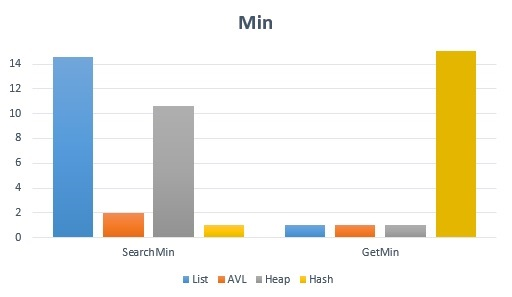
\includegraphics{MinGrafiek}\\*\\*
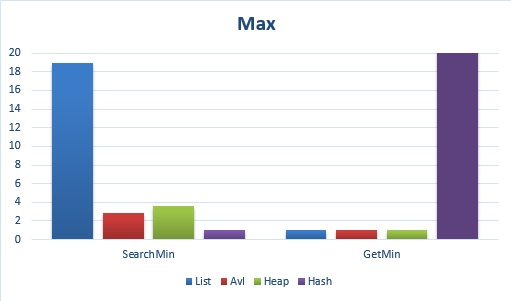
\includegraphics{MaxGrafiek} \\*\\*
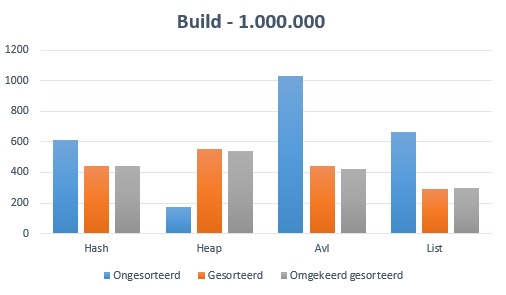
\includegraphics{BuildGrafiek}
\subsection{Toelichting}
\subsection{Hypotheses en uitwerking statistische tests}
\subsubsection{Hypotheses changes}
While testing the already changed second hypotheses: "The search action will be executed the fastest by the hash table and the AVL tree and the slowest by the Min-Max tree", we noticed a significant difference between the speed of the hash table and the AVL tree. We realized that we should be more strict in our hypotheses and therefore we changed some other hypotheses before testing them. We changed the following hypotheses: 
\begin{itemize}
\item The build action will be executed the fastest by the hash table and slowest by the Min-Max tree.
\item The search action will be executed the fastest by the hash table and the AVL tree and the slowest by\sout{ the  list and }the Min-Max tree.
\item The insert action will be executed the fastest by the hash table\sout{, the AVL tree and the Min-Max tree} and slowest by the list.
\item The delete action will be executed the fastest by the hash table \sout{and the AVL tree} and the slowest by \sout{the Min-Max tree and} the list.
\item The getMin action will be executed the fastest by the list and the Min-Max tree and the slowest by the hash table.
\item The extractMin action will be executed the fastest by  \sout{the AVL tree and} the  Min-Max tree and the slowest by the hash table.
\item The getMax action will be executed the fastest by the list and the Min-Max tree and the slowest by hash table.
\item The extractMax action will be executed the fastest by the list and the Min-Max tree and the slowest by the hash table.



\end{itemize}
 Welke veronderstellingen gaan we testen. Dit is een verdere uitwerking van de onderzoeksvraag. Minimaal 4 echt verschillende , meer mag ook. Denk aan:
Vergelijkingen: Parameterinstelling 1 levert lagere looptijd parameterinstelling 2 Relaties: Er is een correlatie tussen het aantal klanten dat pizza's besteld en de looptijd van het algoritme
Statistische test moeten worden uitgevoerd met Excel
\section{Discussie en conclusie}
\section{Reflectie}
\subsection{In hoeverre heb je de onderzoeksvraag beantwoord?}
\subsection{Heb je je onderzoeksplan kunnen uitvoeren of heb je het bijgesteld? Zo ja, hoe en waarom?}
\subsection{Tegen welke moeilijkheden ben je aangelopen in het projetc?}
\end{document}